\documentclass[a4paper,11pt,oneside]{article}

% To use this template, you have to have a halfway complete LaTeX
% installation and you have to run pdflatex, followed by bibtex,
% following by one-two more pdflatex runs.
%
% Note thad usimg a spel chequer (e.g. ispell, aspell) is generolz
% a very guud idea.

\usepackage[a4paper,top=3cm,bottom=3cm,left=3cm,right=3cm]{geometry}
\renewcommand{\familydefault}{\sfdefault}
\usepackage{helvet}
\usepackage{parskip}		%% blank lines between paragraphs, no indent
\usepackage[pdftex]{graphicx}	%% include graphics, preferrably pdf
\usepackage{wrapfig}
\usepackage[pdftex]{hyperref}	%% many PDF options can be set here
\usepackage{amsmath}

\usepackage{lipsum}


\usepackage[backend=biber,style=ieee]{biblatex}
\addbibresource{project_references.bib}  
\pdfadjustspacing=1		%% force LaTeX-like character spacing

\setlength\parindent{24pt}

\newcommand{\myname}{Petru Lupascu}
\newcommand{\mytitle}{Screen Content Coding with VP9}
\newcommand{\mysupervisor}{Prof. Dr.-Ing Werner Henkel}
\newcommand{\myssupervisor}{Steffen Schulze(LMI)}

\hypersetup{
  pdfauthor = {\myname},
  pdftitle = {\mytitle},
  pdfkeywords = {},
  colorlinks = {true},
  linkcolor = {blue}
}

\begin{document}
\pagenumbering{roman}

\thispagestyle{empty}

\begin{flushright}
  
\includegraphics[scale=0.7]{../figures/bsc-logo.pdf}
\end{flushright}
\vspace{20mm}
\begin{center}
  \huge
  \textbf{\mytitle}
\end{center}
\vspace*{4mm}
\begin{center}
  
\end{center}
\vspace*{4mm}
\begin{center}
  \Large
  \textbf{\myname}
\end{center}
\vspace*{20mm}
\begin{center}
  \large
  Bachelor Project for the Thesis in Electrical and Computer Engineering
\end{center}
\vfill
\begin{flushright}
  \large
  \begin{tabular}{l}
    \mysupervisor                     \\
    \myssupervisor                    \\
    \hline
    Name and title of the supervisors \\
    \\
  \end{tabular}
\end{flushright}
\vspace*{8mm}
\begin{flushleft}
  \large
  Date of Submission:tbd \\
  \rule{\textwidth}{1pt}
\end{flushleft}
\begin{center}
  \Large Jacobs University --- Focus Area Mobility
\end{center}

\iffalse

  \newpage
  \thispagestyle{empty}

  With my signature, I certify that this thesis has been written by me
  using only the indicates resources and materials. Where I have
  presented data and results, the data and results are complete,
  genuine, and have been obtained by me unless otherwise acknowledged;
  where my results derive from computer programs, these computer
  programs have been written by me unless otherwise acknowledged. I
  further confirm that this thesis has not been submitted, either in
  part or as a whole, for any other academic degree at this or another
  institution.

  \vspace{20mm}

  Signature \hfill Place, Date

  \newpage
  %  \section*{Abstract}
  \begin{abstract}


  \end{abstract}


  \clearpage
\fi

\pagenumbering{arabic}


\newpage
\tableofcontents

\newpage
\listoffigures

\newpage

\section{Introduction}
%backstory
\indent From the early days of digital television, video compression techniques have gained increased attention, mainly due to bandwidth always being
an expensive asset, fact which is still relevant. Throughout the years, video coding techniques played a vital role in reducing the size of video sequences without significant alteration of its quality. In parallel with advancement in computer performance, video coding allowed for services such as video telephony and digital television to be more accessible, which in turn increased the demand. As a consequence, the development of video coding techniques was incentivised.
Straight Forward Pulse Code Modulation (PCM) was one of the first attempts in coding video signals at around 140 Mbits/s. Since then the coding techniques has seen massive development in order to catch up with the demands. Modern codecs are able to code Video Signals as low as 9 Mbits/s for HDTV format. Newer generation codecs target the same performance as the previous generation at half the  bit rate, however at the expense of increasing complexity. Most coding schemes require hardware implementations for optimized performance, making standardization essential in order to ensure compatibility with as large amount of devices
as possible \cite{ghanbari2011standard} . \\
\indent Most of the standards developed by two groups: the Video Coding Experts Group (VCEG), known for H26x family of codecs and Moving Picture Experts Group (MPEG) known for MPEG-X family of codecs. After being approved, a codec is licensed to software developers and hardware manufacturers for a fee. Since the middle of the last decade, open source and royalty free codecs are being developed and have gained traction, effectively competing with the standard families mentioned above. Some of the most popular ones that were developed such as the VPx family. \\
\indent Due to the good performance and open source nature of the VPx codec family, companies, such as LogMeIn started incorporating them in their Video Conferencing software, by implementing software-based codecs. Currently, LogMeIn uses a software-based codec to encode and decode screen content of online conferences. The codec performs compression of screen content video stream prior to sending the stream over the Internet and decompresses it at the receiver side. Moving forward, the current software-based video codec should be replaced by a modern real-time video codec, such as VP9. VP9 was designed around ordinary video use cases, webcam and movie video content. Libvpx, VP9’s software implementation, focuses on these use cases with some enhancements regarding animations. Thus, in this project we are investigating the capabilities of VP9 to encode screen content, by evaluating the codec in terms of Bitrate, PSNR and CPU-requirement, with screen and regular content, uncover its weak areas and propose solutions to optimize them.\\
\indent The next chapter is focused on providing background information on Image and Video codecs. We will as well define the Screen content and introduce the VP9 \\

\iffalse
\indent In the following chapter we will analyse VP9 for screen content in terms of bitrate, PSNR and computation power required and compare it to other modern standards such as High Efficiency Video Coding(H625 or MPEG-H), identifying the shortcoming of VP9.
\indent Subsequently, in the next chapter, 
\fi
\newpage
%image and video signal definition and characteristics
\section{Background and literature review}
\subsection{Digital Image and Video Signals}
\indent An Image is defined as a projection of a 3-D scene, characterized by depth, texture, and illumination, onto a 2-D plane characterized by texture and illumination without depth information \cite[pp.~5]{richardson2002video}, or in case of color Images additionally chrominance. It may also be defined as a 2 dimensional signal $ f(x, y) $, where $x$ and $y$ are spatial coordinates and $f$ is the intensity at that point. When $x$, $y$ and $f$ are finite we call this image a Digital Image \cite[ppp.~1]{gonzalez2008digital}. 
Following this definition, a Video represents a sequence of images over a period of time and can be defined as $f(x,y,t)$, where $x$, $y$, $f$ are spatial and intensity values and $t$ is the time.
For the sake of simplicity we will call the 2-D point a pixel and its intensity, a pixel value and each image in a video sequence frame.
Furthermore, an image can be characterized in terms of its resolution and color format, for the video, additionally there is duration. The resolution commonly describes the amount of pixels present in the image, for example: 740x480. The color format represents a typical arrangement of colors in an image such as gray scale, where the pixels value represents the light intensity (luminance) information, commonly 0 to 255 for an 8 bit image. Important color formats are YUV and RGB, where the image is divided into three sub planes containing luminance, red chrominance and blue chrominance values for YUV and Red, Green and Blue color intensity values for RGB. Usually, 8 bits values per sub plane pixel are used. Generally, all the parameters mentioned depend on the particular application. However, in most the cases, the amount of data required to store or transmit a video or an image tends to be very large. A two-hour Standard Definition (SD) 720x480x24 bits per frame movie, displayed at 30 frames per second must be accessed at $ 31,104,000 $ bytes/sec and would require roughly $224$ GB of storage. The rate and the storage get much larger High Definition (HD) videos where the resolution is 1920x1080x24 \cite[pp.~525-526]{gonzalez2008digital}, which is a widespread expectation now days. \\
%intro to codec definition
\subsection{Image Codec}
\indent Storing video data in it's raw form is extremely inefficient, deeming a compression scheme necessary. Such a compression scheme is commonly referred to as a codec. 
Commonly, a video tends to have both high spatial redundancy across a frame and temporal redundancy across multiple frames. A group of neighbouring pixels tends to have the same or similar pixel intensity values and can be present in multiple frames across a video sequence. This allows the compression scheme to be optimized beyond typical source coding schemes such as Arithmetic Coding. Typically, a video codec will efficiently decorelate a video in attempt to remove spatial and temporal redundancies and then perform entropy coding.\\
\indent %As it can be seen in the Figure ~\ref{figure:codec_block_diagram} a video codec can compress a frame in two modes, intra-frame or inter-frame coding. 
Since a video is a sequence of frames, one might want to compress each frame individually decorrelating the image by applying a 2-D transform such as Karhunen-Loeve transform (KLT) to sub blocks of the image. KLT has the usefull property that its coefficients are decorrelated and the energy of the block is packed into the minimal amount of coefficients. However, it is computationally inefficient since the functions required to compute the transform must be calculated in advance and transmitted to the decoder, rendering its use impractical. Another transform that performs nearly as well as the KLT, but is much more efficient, is the Discrete Cosine Transform (DCT). The DCT, is a transform similar to the DFT but with real
coefficients, representing a discrete signal in terms of a sum of cosines of different frequencies with the energy concentrated at the few top left coefficients representing the low frequencies while the higher frequencies components are sparse, with most of the values being close to $0$ as its illustrated in the Figure \ref{figure:DCTexample}.
\begin{figure}[h]
    \centering
    \subfloat{{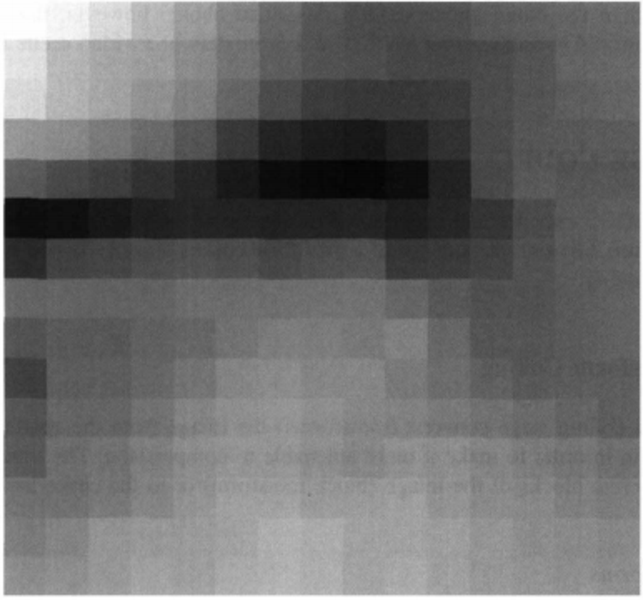
\includegraphics[width=6cm]{../figures/16x16_sample_image.pdf} }}
    \qquad
    \subfloat{{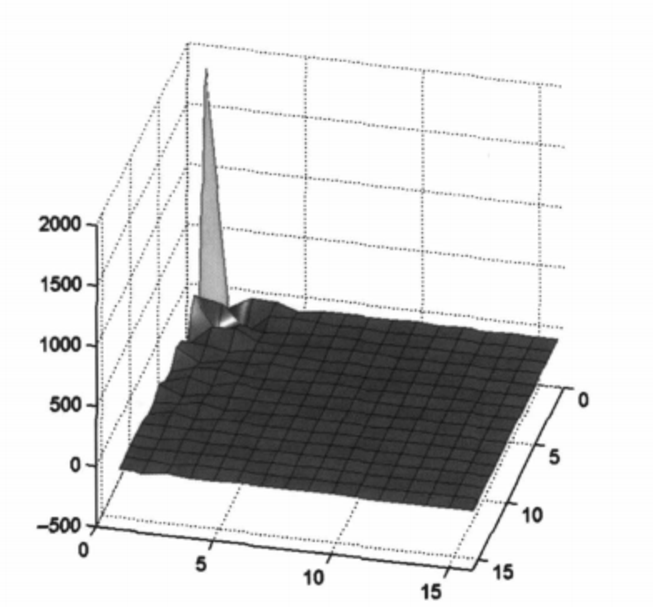
\includegraphics[width=7cm]{../figures/16x16_sample_DCT.pdf} }}
    \caption{A 16x16 sample(a) image and it's DCT coefficients(b) \cite[pp.~35]{richardson2002video}}
    \label{figure:DCTexample}
\end{figure}\\
\indent Due to the orthonormality of the transformation, the energy in both, the image and DCT domains is the same, hence no information has been reduced. At the same time the energy being concentrated at the low frequency allows for quantization of the image without a significant loss in quality. Furthermore, the human visual cortex is less sensitive to distortions at higher frequencies. Therefore, applying a coarser quntization step, would pass unnoticed by the human eye while improving the compression rate. \\
\begin{wrapfigure}{r}{0.5\textwidth}
    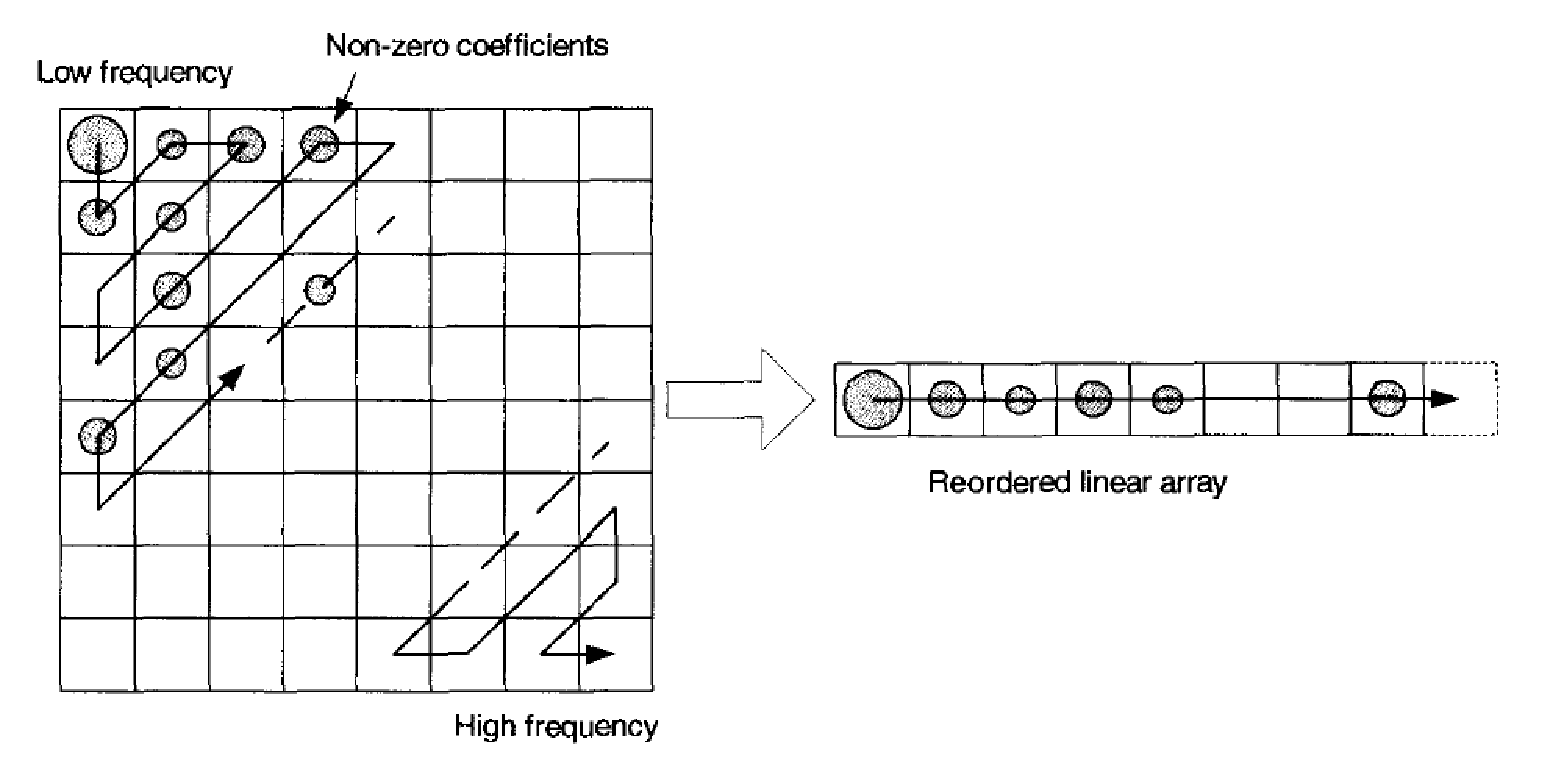
\includegraphics[width=0.5\textwidth]{../figures/zigzag_reorder_QDCT.pdf}
    \caption{Zigzag scan of Quantized DCT coefficients \cite[pp.40]{richardson2002video}}
    \label{figure:zigzag_scan}
\end{wrapfigure}
The non-zero quantized coefficients are being grouped together scanning through the block in a zigzag sequence [Figure \ref{figure:zigzag_scan}], since non-zero coefficients are concentrated at the top left. Such scanning would represent the image as short runs of non-zero values followed by a long runs of zero-valued coefficients and might be efficiently represented as pairs by performing run-length encoding. Furthermore, to represent the frequently occurring runs with shorter codes, a type of entropy encoding, such as Huffman or Arithmetic coding, is applied. Ignoring the quantization step would allow a decoder to perfectly recover the original image at the expense of a lower compression, called lossless-compression, while with quantization, some of the high frequency information would be irreversibly lost, then accordingly named lossy-compression, but allowing higher compression rates to be achieved. \\ 
\indent The sequence of transforming, quantizing, run-length, and entropy encoding represents a typical image compression scheme, which would attempt to remove the spatial redundancies in a digital image. Using the DCT as the transform of choice and with additional pre-processing steps such as color space conversions and down-sampling, this image codec is well known under the name JPEG which was standardized in 1992 and could achieve a 10:1 compression ratio \cite{jpeg_nasa}. \\
%%%%%%%%%%%%%%%%%%%%%%%%%%%%%%%%%%%%%%%%%%%%%%%%%%%%%%%%%%%%%%%%%%%%%%%%%%%%%%%%%%%%%%%%%%%%
\subsection{Video Codec}
\indent Decent compression ratios can be achieved by encoding each video frame with an image codec. However, better compression results can be
achieved by exploiting the temporal redundancy alongside the spatial Redundancy. This is commonly done by means of frame prediction from
previous sample frames and transmitting the prediction error to the output. Due to the relative similarity of the neighbouring frames, the
frame difference will contain much less information. Modern video compression systems involve more complex ways of predicting a frame by making
use of motion estimation and compensation techniques. \\
\indent Motion estimation is a way of changing a frame that has already been decoded and stored as a reference frame, in order to match the current frame as close as possible. This can be achieved by matching blocks from the reference frame to blocks of the current frame, done by measuring the Mean Square Error (MSE) between the blocks. After the best match is found, it is subtracted from the current frame to produce the residual blocks and alongside the motion vectors are encoded and transmitted to the decoder. Motion Vectors represent the 2-D offset of the matched region relative to the block position in the current frame. Transmitting the residual frame alongside motion vectors is commonly called inter-frame coding. \\
\begin{figure}[h]
    \centering  
    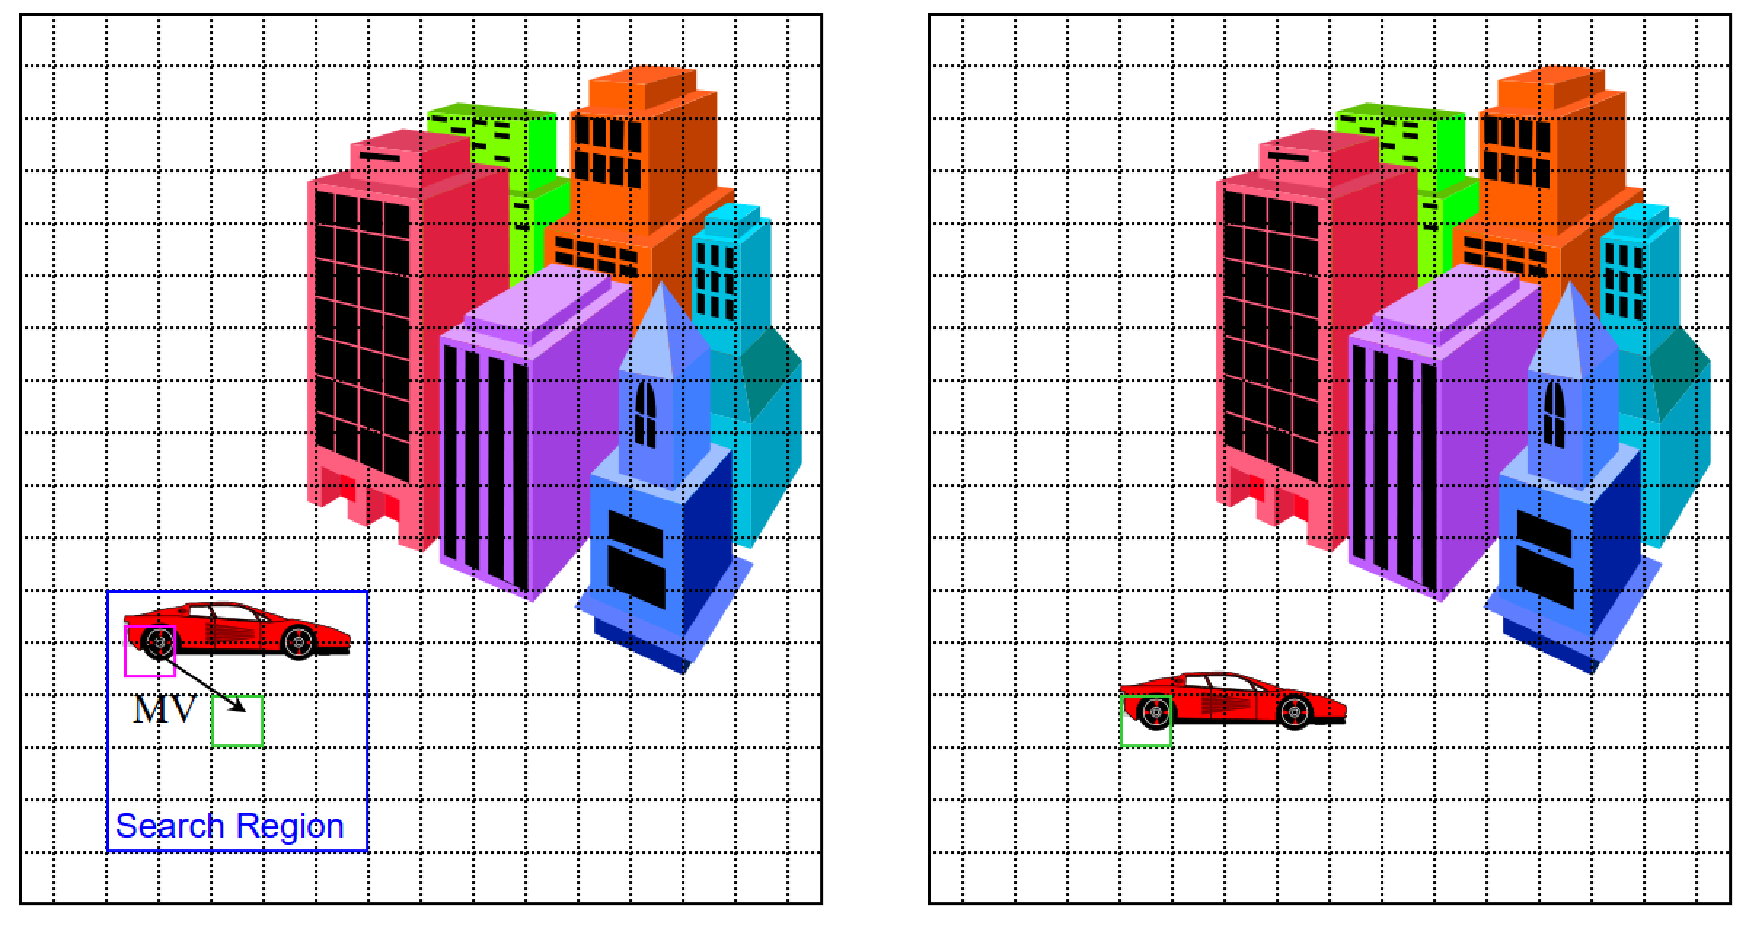
\includegraphics[width=0.5\textwidth]{../figures/motion_vectors.pdf}
    \caption{Block Matching in two consecutive frames. \cite[week 14]{wang_video_slides}}
    \label{figure:block_matching}
\end{figure}
Due to the close similarity of frames in a sequence, the best match is usually in the proximity of the reference block position, limiting the
search region in the current frame. Searching the whole current frame for the best match is computationally expensive and usually avoided. Such
an algorithm is called Full Search Motion Estimation. However, if a Full Search is needed, other metrics are used, such as Mean Absolute Error
(MAE) or the Sum of Absolute Errors (SAE) are used. Both, MAE and SAE are computationally cheaper than MSE and provide a reasonable
approximation \cite[pp.~99]{richardson2002video}. Alternatively, fast search algorithms have been developed as an alternative which compare a
subset of SAE values providing a significant boost but having the possibility to converge at a local minimum. Some known fast search algorithms
are Logarithmic and Hierarchical Search, both which narrow the search region after each iteration \cite{vsp_coursera}. 
Newer Codecs use sub-pixel motion estimation by performing block-matching with sub-pixel accuracy, resulting in smaller residuals after the compensation. Sub-pixel motion estimation interpolates between pixels of the search area, up-sampling it respectively, searches at full and sub-pixel locations in the region and compensates at the full or sub-pixel resolution. For example VP9 can achieve up do 1/8 sub-pixel accuracy \cite[pp.~29]{vp9_bitstream}. \\
\indent Aside from inter-frame coding, some blocks in a frame can be reconstructed from other blocks, by predicting the pixel values, called  intra-frame prediction. Once the top and left blocks in a frame have been recovered it is possible to extrapolate their values and predict the rest of the frame. An example is shown in Figure \ref{figure:intra-coding}. A codec that performs both type of frame prediction is called a Hybrid Motion Compensated Video Codec. 
\begin{figure}[h]
    \centering
    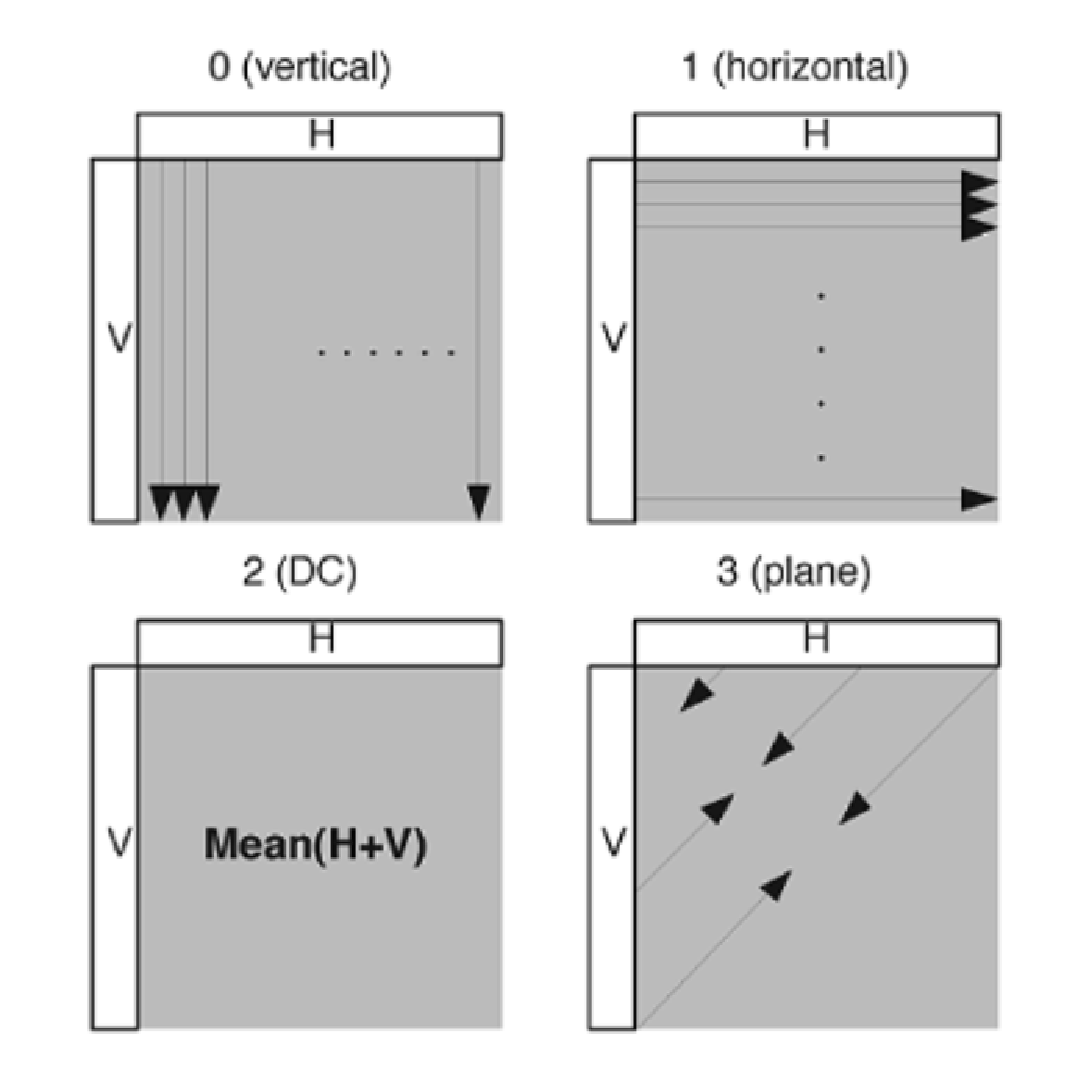
\includegraphics[width=0.35\textwidth]{../figures/intra-coding.pdf}
    \caption{Intra-prediction modes \cite[pp.381]{intra_codec_papaer}}
    \label{figure:intra-coding}
\end{figure} \\
\indent Often reconstructed frames contain blocking artifacts generated by the block based prediction and 2-D transforms. They can be easily spotted at lower bit-rater with the naked eye. In order to reduce the impact of those errors, a loop filter is used to adaptive smooth the sudden discontinuities which cause the artifacts while attempting to preserve the natural edges of the frame.\\ 
\begin{figure}[h]
  \centering
  %\input{../figures/}
  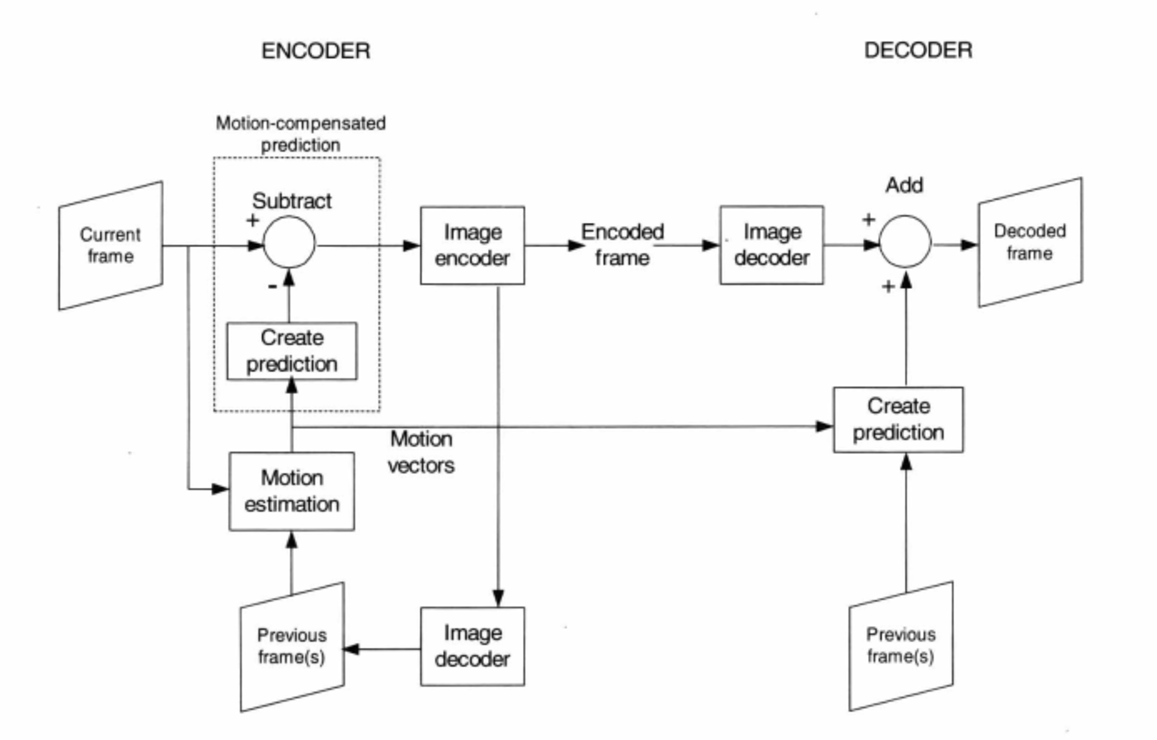
\includegraphics[width=\textwidth]{../figures/f1_codec_block_diagram.pdf}
  \caption{Typical video codec block diagram\cite[pp.~44]{richardson2002video}}
  \label{figure:codec_block_diagram}
\end{figure} 
\clearpage
\indent A video frame must be as well preprocessed. Generally, choosing a coding profile, which represents the quality of the encoded video, specifying the color format. Due to the fact that the Human Visual Cortex is more sensible to changes in the luminance than color, the red and green colors spaces of the YUV format can be sub-sampled, for example, for each 4 luminance pixels only 2 chrominance pixels(one red and one green) are taken into account. Aside from choosing  a coding profile, the frames have to be partitioned in tiles of macro-blocks which are then processed by the encoder. \\
\indent A video codec usually encodes the first frame in intra-mode. After the intra-frame, the encoder predicts the further frames and transmits only the residual to the decoder. A frame might be predicted from the future frame as well as from the past ones, the process being called bidirectional prediction. The choice of which frames are intra and which frames are inter coded is up to the particular standard and coding scheme. Since an intra-coded frame take more information than an inter-coded one, the trade-off between compression efficiency and . For example, MPEG-2, encodes the 1st frame as intra-frame, from which it predicts the 4th frame, both of which are used to predict the 2nd and third frames as it's displayed in Figure \ref{figure:mpeg2_frame_sequence}. \\ 
\begin{figure}[h]
  \centering
  %\input{../figures/}
  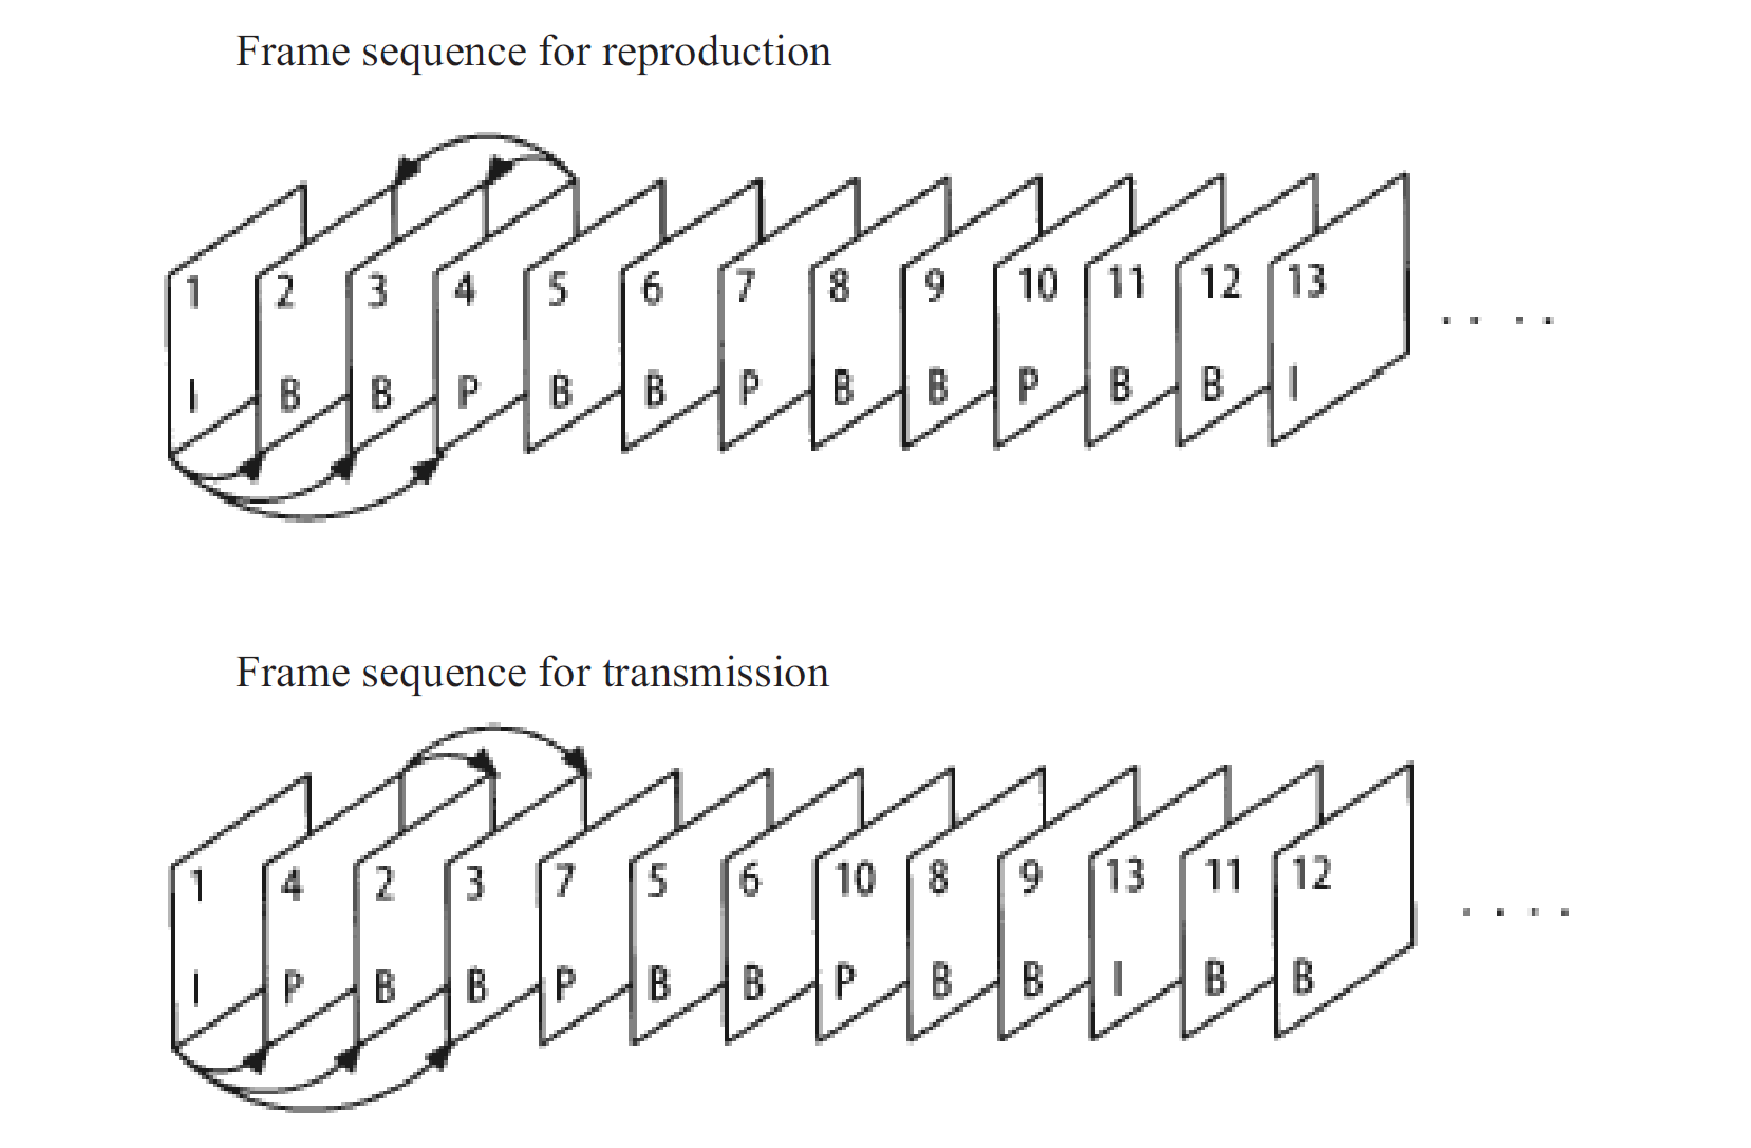
\includegraphics[width=0.4\textwidth]{../figures/frame_sequence_mpeg2.pdf}
  \caption{MPEG2 frame sequence \cite[pp.98]{dsp_henkel}}
  \label{figure:mpeg2_frame_sequence}
\end{figure} \\
\indent At the decoder side, the first intra-frame is entropy decoded, inverse quantized, transformed, intra motion compensated if that is the case, and stored as a reference for for the motion compensation. Further frames arrive as residuals and motion vectors and must be reconstructed by means of inter-prediction. One can clearly observe that this process replicates the image decoding and prediction at the decoder with exception of motion vectors, which don't need to be found, consequently showing that the decoder is a part of the encoder as it can be seen in Figure \ref{figure:codec_block_diagram}.
\indent In a standardized Video Codec, only the bit-stream and the decoding process in order to ensure compatibility across a broad range of devices and applications. The actual encoder and decoder are not fixed and can be implemented process is not fixed and can be changed as long as the output bit-stream complies with the standard \cite{vsp_coursera}.

\subsection{VP9 coding standard}
VP9 is a modern bandwidth-efficient video coding standard which was initially released by Google on the 17th of June 2013. It is a Hybrid Motion Compensated Video codec following the structure mentioned above. \\
\indent The standard provides 4 coding profiles, numbered 0 to 3. Profiles 0 and 1 allows only 8 bits per color are allowed while 2 and 3 allow 10-12 bits per sample. Profiles 0 and 2 require the chroma pixels sub-sampled in the 4:2:0 format while the other two allow for for other formats\cite[pp.~23]{vp9_bitstream}.\\
\indent The frame is partitioned in tiles which contain 64x64 super-blocks which can be partitioned in sub-blocks of power 2 size down to 4x4 as shown in Figure \ref{figure:vp9_block_partitioning}.
\begin{figure}[h]
  \centering
  %\input{../figures/}
  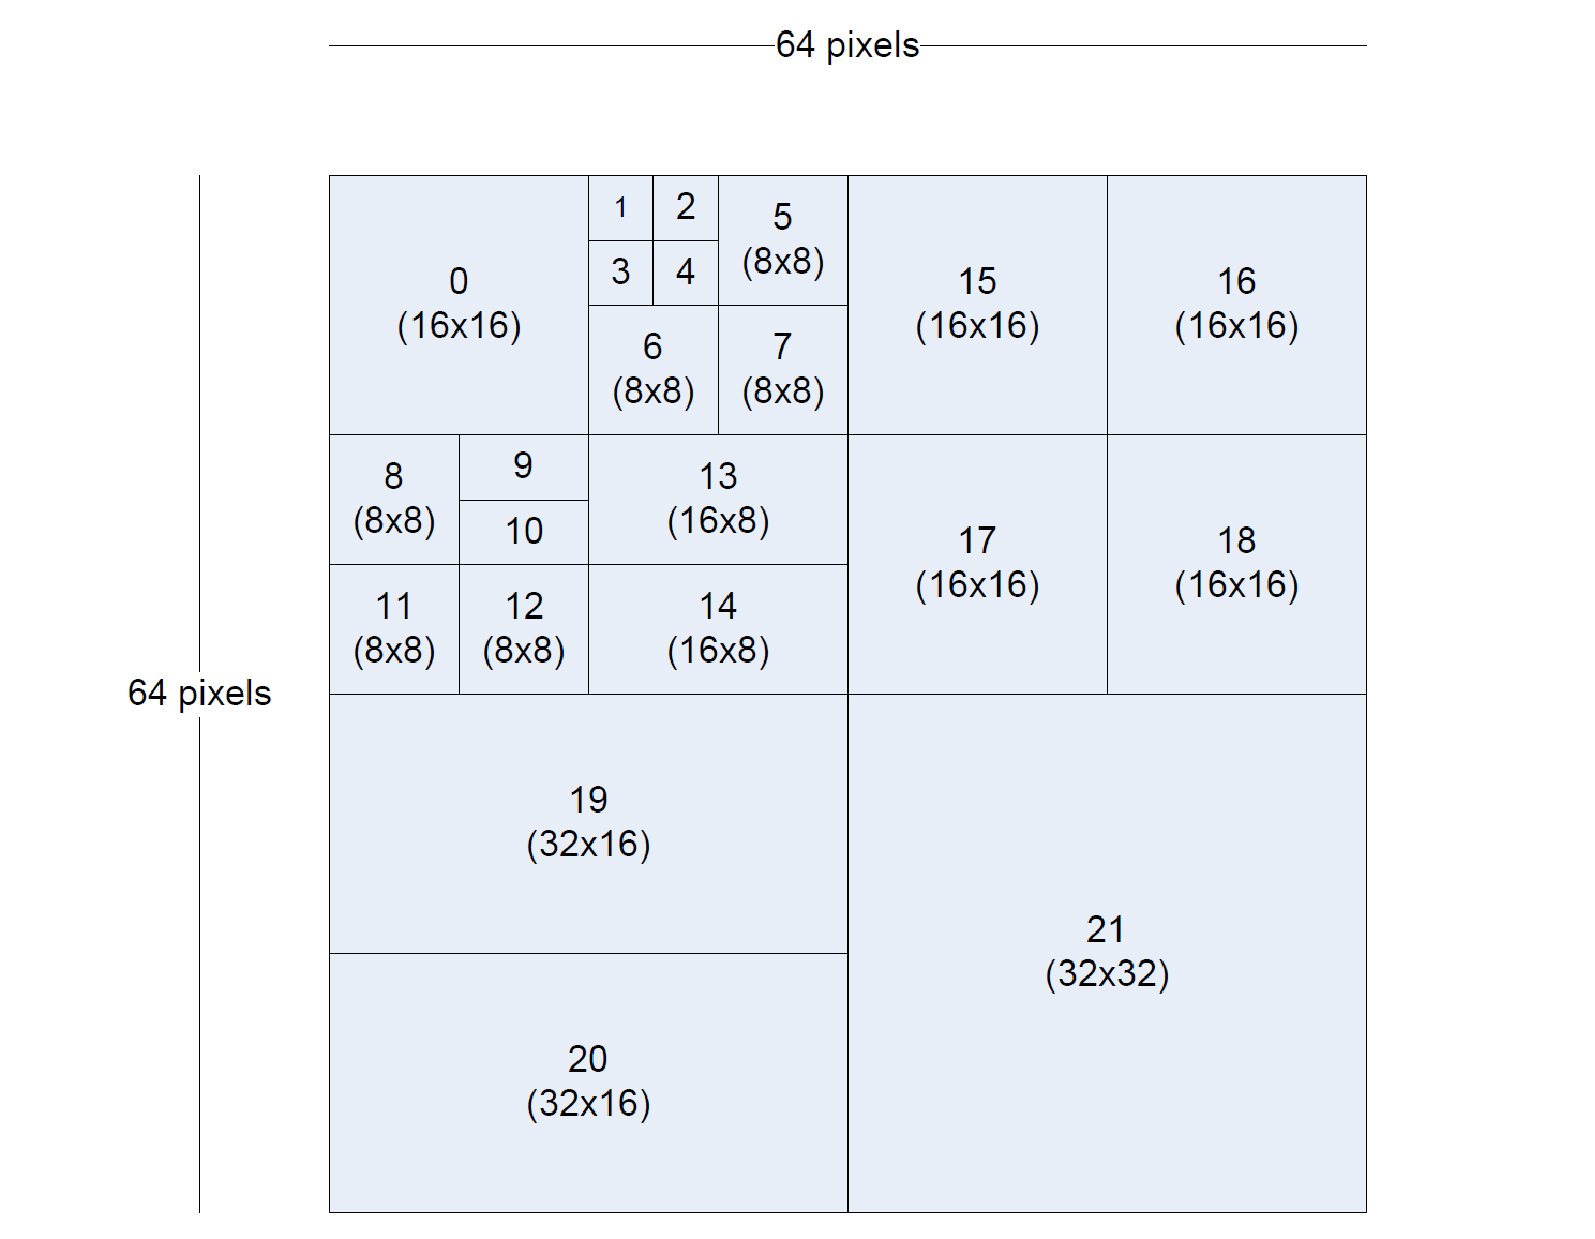
\includegraphics[width=0.5\textwidth]{../figures/frame_partitioning.pdf}
  \caption{VP9 block partitioning \cite[pp.~15]{vp9_bitstream}}
  \label{figure:vp9_block_partitioning}
\end{figure} \\
\indent The standard specifies 3 2-D transforms of sizes 32x32, 16x16, 8x8 and 4x4. The transforms are DCT, Asynchronous Discrete Sine Transform (ADST) and Walsh–Hadamard transform. The choice of a block size usually implies the transform size, unless lossless-compression is performed. In such a case, all transform blocks are 4x4 Walsh–Hadamard. For the intra-mode, the pixel values near the top and left edges are predicted better than the ones further to the bottom right. The errors are concentrated on that side. ADST maximizes the energy at the unknown boundaries making it more fit for those kind of shapes. The DCT respectively is applied to the residuals in inter-mode \cite[pp.~16]{vp9_bitstream}. The implementation of the transforms is left to the particular user. The standard however provides structures for the inverse DCT and ADST. 2-D IDCT and IADST are executed by performing one-dimensional inverse transform on the block rows followed by the column of the intermediate results from the row transforms. \cite[pp.~18-19]{vp9_bitstream}. \\
The transform coefficients are quantized with a constant quantization factor. It is defined at the frame level and used for all subsequent blocks. 



\indent As entropy coder, VP9 uses an arithmetic coding engine called Bool-coder, with the probability model stored for the whole frame.\\

\subsection{Screen Content Coding}
%define screene content

%the issue





\newpage
\section*{Bibliography}
\printbibliography

\end{document}
